%%This is a very basic article template.
%%There is just one section and two subsections.
\documentclass{scrartcl}

\usepackage[T1]{fontenc}
\usepackage[utf8]{inputenc}
\usepackage[ngerman]{babel}
\usepackage{lmodern}
\usepackage{amsmath}
\usepackage{amsfonts}
\usepackage{hyperref}
\usepackage{graphicx}


\hypersetup{
pdfborder = {0 0 0},
urlbordercolor = {0 0 0},
colorlinks = true,
linkcolor = black,
citecolor = black,
filecolor = black,
urlcolor  = black
}

\title{Software Challenge 2013 - Cartagena}
\subtitle{Spielregeln}



%% Variablen
\newcommand{\SpielSegmenteAnzahl}{\emph{5}}
\newcommand{\KartenAnzahl}{\emph{KartenAnzahl}}
\newcommand{\PiratenAnzahl}{\emph{6}}
\newcommand{\EmptyPlainPage}{\newpage\thispagestyle{plain}\ \newpage}
\newcommand{\RundenAnzahl}{\emph{30}}

\begin{document}
\maketitle

\begin{figure}[h]
	\centering
	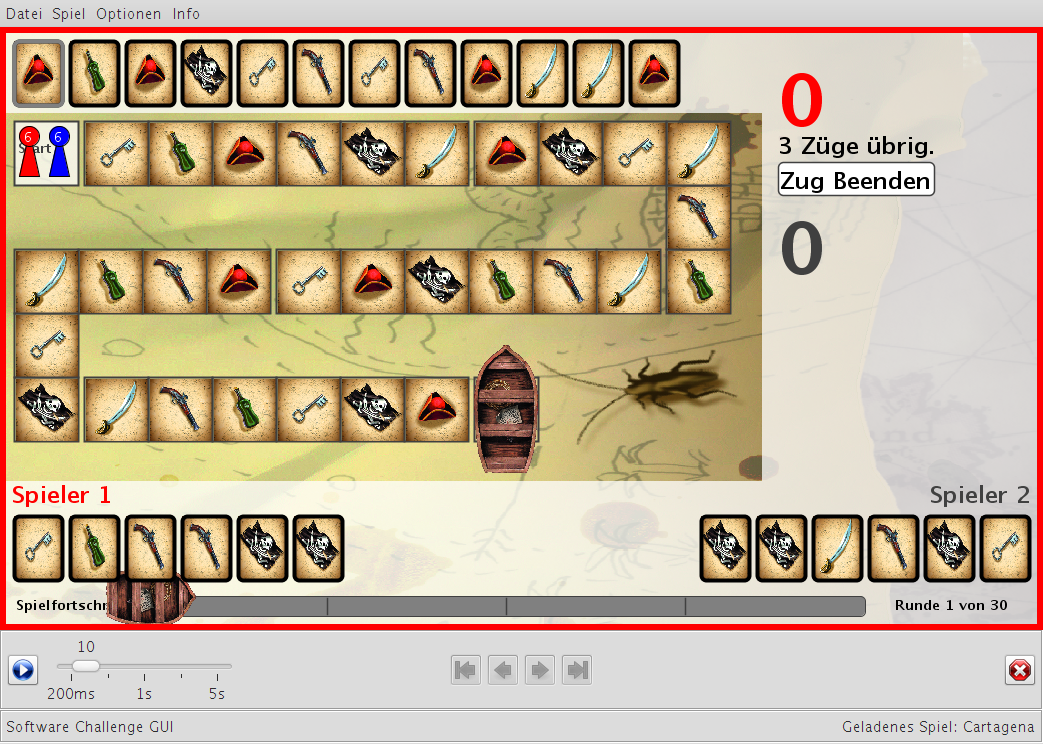
\includegraphics[width=\linewidth]{bilder/Uebersicht.png}
\end{figure}

"Die Nutzung des Spielkonzeptes "Cartagena" (Name, Spielregeln und Grafik)
erfolgt mit freundlicher Genehmigung der Winning Moves Deutschland GmbH."
\newpage
\tableofcontents
\EmptyPlainPage

\section{Einführung}
Das Spiel der Softwarechallenge 2012 ist eine abgewandelte Version von Cartagena
des \emph{Winning Moves} Verlages. Hierbei werden Piraten abwechselnd, mithilfe
von Zugkarten über das Spielfeld bewegt.\\

Ziel des Spiels ist es alle Piraten auf die Schaluppe zu bringen. Wer dies als
Erstes schafft, gewinnt das Spiel.
\begin{itemize}
  \item Cartagena in abgewandelter Tortuga Version
  \item Ziel : Alle Piraten auf die Schaluppe
\end{itemize}

\section{Spielmaterial}
	\subsection{Das Spielfeld}
	Das Spielfeld setzt sich aus \SpielSegmenteAnzahl\ Segmenten zusammen,
	innerhalb derer die Symbole \emph{Schlüssel}, \emph{Flasche}, \emph{Hut},
	\emph{Pistole}, \emph{Flagge} und \emph{Säbel} jeweils genau einmal vorkommen.
	Die Reihenfolge ist innerhalb jedes Segmentes und von Spiel zu Spiel zufällig.
	Das Spielfeld wird durch ein Start- und ein Zielfeld ergänzt.
	Auf einem Spielfeld dürfen, mit Ausnahme von Start- und Zielfeld jeweils
	maximal 3 Spielfiguren stehen.
	\subsection{Die Spielsteine}
	Jeder Spieler startet mit \PiratenAnzahl\ Piraten im Startfeld, welche alle ins
	Ziel gebracht werden müssen.
	\begin{figure}[h]
		\label{fig:Spielfeld}
		\centering
		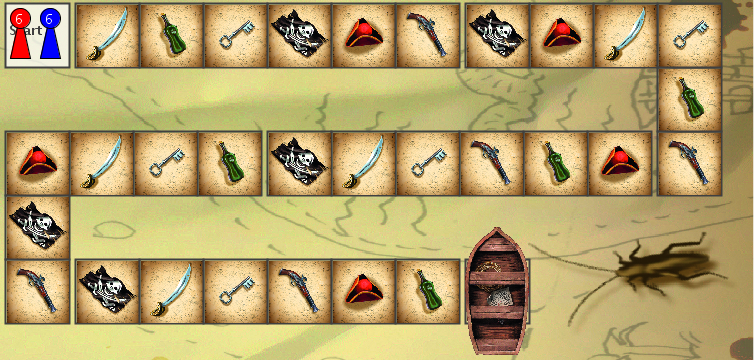
\includegraphics[scale = 0.5]{bilder/Spielfeld}
		\caption{Ein mögliches Spielfeld.}
	\end{figure}
	
	\subsection{Die Spielkarten}
	
	\begin{figure}[h]
		\centering
		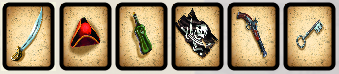
\includegraphics[scale = 0.5]{bilder/Karten}
		\caption{Die Spielkarten mit Symbolen}
	\end{figure}
	Zum Ziehen der Piraten werden die Spielkarten benötigt. Die Karten tragen
	analog zu den Spielfeldern wieder die Symbole \emph{Schlüssel}, \emph{Flasche}, \emph{Hut},
	\emph{Pistole}, \emph{Flagge} und \emph{Säbel}.\\
	Insgesamt gibt es 102 Karten, also 17 von jedem Symbol. Jeder Spieler startet
	mit 6 Karten auf der Hand und darf maximal 8 Karten auf der Hand halten.\\
	In der oberen Leiste werden die nächsten 12 Karten angezeigt, welche als
	nächstes gezogen werden können. Die Reihenfolge geht von links nach rechts.\\
	Sind alle Karten verbraucht, so werden die Karten vom Ablagestapel gemischt und
	neu bereitgelegt.
\section{Spielablauf}
	Es beginnt der Rote Spieler. Jeder Spieler darf innerhalb einer Runde 3 Züge
	machen. Diese dürfen aus einer beliebigen Kombination von Vorwärts- und
	Rückwärtzügen bestehen.\\
	Bei einem Vorwärtszug muss eine Karte von der Spielerhand abgelegt werden, bei
	Rückwärtzügen können neue Karten vom Stapel gezogen werden.
	
	\begin{figure}[h]
		\label{fig:PossibleMoves}
		\centering
		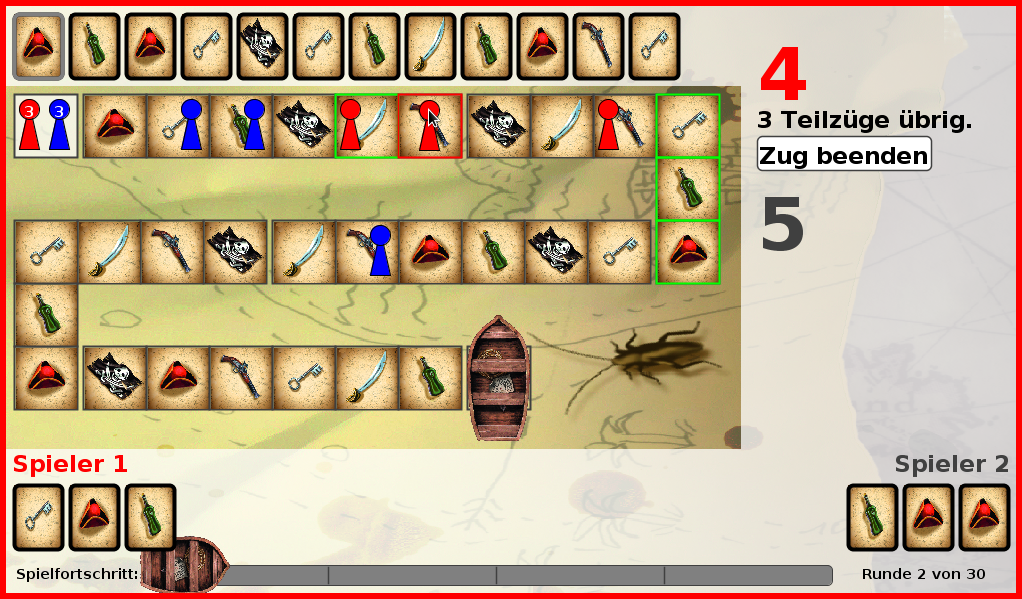
\includegraphics[width=\linewidth]{bilder/Moves}
		\caption{Eine Spielsituation, in der sowohl Vorwärts- als auch Rückwärtszüge
		möglich sind.}
	\end{figure}
	\subsection{Vorwärtszüge}
	Bei einem Vorwärtszug wählt ein Spieler ein Feld auf dem sich eine oder mehrere
	Spielfiguren der eigenen Farbe befindet. Zum Vorwärtsziehen muss eine Karte
	abegelegt werden und die Spielfigur zieht auf des nächste unbesetzte Feld,
	welches das gleiche Symbol, wie die Karte zeigt. Alle übrigen Felder, sowie
	einfach oder mehrfach besetzte Felder werden hierbei übersprungen.\\
	Gibt es zwischen einem Piraten und der Schaluppe kein Feld mehr mit dem auf
	einer Karte abgebildeten Symbol, oder sind alle Felder mit diesem Symbol
	belegt, so kann durch ablegen dieser Karte direkt auf das Zielfeld gezogen werden.
	\begin{figure}[h]
		\centering
		\label{fig:Zielfeld}
		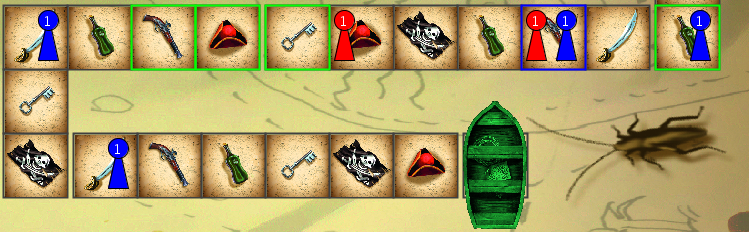
\includegraphics[width=\linewidth]{bilder/zielfeld}
		\caption{Alle Säbelfelder sind belegt. Durch Ablegen einer Säbelkarte kann
		ins Zielfeld gezogen werden.}
	\end{figure}
	\subsection{Rückwärtszüge}
	Durch Rückwärtszüge können neue Karten vom offenen Kartenstapel gezogen werden.
	Hierbei wählt ein Spieler eine Spielfigur aus und zieht sie auf das nächste
	zurückliegende Feld, auf dem bereits entweder eine oder zwei Spielfiguren
	stehen. Das Startfeld ist hierbei ausgeschlossen und es ist egal welche Farbe
	die Spielsteine auf dem zurückliegenden Feld haben.\\
	Stehen auf dem zurückliegenden Feld 2 Piraten, so zieht der Spieler 2 neue
	Karten vom offen Stapel, sonst darf er nur eine Karte ziehen.
	\subsection{Punkteverteilung}
	Die Punkte ergeben sich aus der Anzahl der Piraten, welche sich im jeweiligen
	Segment befinden. Hat ein Spieler beispielsweise zwei Piraten in Segment 1 und
	einen Piraten in Segment 3, so ergibt sich eine Gesamtpunktzahl von 4.\\
	Spielsteine auf dem Startfeld bringen keine Punkte und ein Pirate im Zielfeld
	bringt 6 Punkte.
\section{Ende des Spiels}
	Hat ein Spieler alle seine Piraten im Zielfeld, so gewinnt dieser. Schafft dies
	keiner der beiden Spieler alle Piraten innerhalb der \RundenAnzahl\ Runden, so
	gewinnt der Spieler mit den meisten Punkten.
\section{Die graphische Benutzeroberfläche}
	
\end{document}
